%\ifx\wholebook\relax\else
%\documentclass[twoside]{book}
%\usepackage[active]{srcltx}
%\usepackage[LY1]{fontenc}
%\usepackage{url}
\makeatletter
\def\url@leostyle{%
  \@ifundefined{selectfont}{\def\UrlFont{\sf}}{\def\UrlFont{\sffamily}}}
\makeatother
% Now actually use the newly defined style.
\urlstyle{leo}

\usepackage{graphicx}
\def\etc{{\textit etc}}
\def\eg{{\textit e.g.}}
\def\ie{{\textit i.e.}}
\def\cf{{\textit c.f.}\ }
\def\erf{\mathop{\textrm erf}}
\def\sign{\mathop{\textrm sign}}
\def\prob{\mathop{\textrm Prob}}
\def\var{\mathop{\textrm var}}
\def\mod{\mathop{\textrm mod}}
\def\cor{\mathop{\textrm cor}}
\def\cov{\mathop{\textrm cov}}
\def\cl{\mathop{\textrm CL}}
\def\kg{\mathop{\textrm Kg}}
\def\patstyle#1{{\textsc #1}}
\def\th{^{\mathop{\textrm th}}}
%\def\st#1{^{\mathop{\rm #1}}}
\def\note#1{\begin{quote}{\textbf Note:} #1\end{quote}}
\def\braket#1{\left\langle #1\right\rangle}
\def\order#1{\let\o=#1{\cal O}\ifx\o 1$\left(n\right)$\else$\left(n^{#1}\right)$\fi}
%\newtheorem{privListing}{Listing}[chapter]
%\newenvironment{listing}{\vskip 3ex\hrule\vskip 1ex\begin{privListing}}{\end{privListing}\hrule\vskip 1ex}
\newtheorem{privExample}{Code example}[chapter]
\newenvironment{codeExample}{\begin{privExample}\begin{quote}\tt}{\end{quote}\end{privExample}}
\def\relboxl#1#2{\hbox to #1\hsize{#2\hfil}}
\def\relboxc#1#2{\hbox to #1\hsize{\hfil #2\hfil}}
\def\relboxr#1#2{\hbox to #1\hsize{\hfil #2}}
\def\transpose#1{{\bf #1}^{\mathop{\rm T}}}
\def\inverse#1{{\bf #1}^{-1}}
%\def\tm{$^{\mathop{\rm TM}}$}
\def\tm{ }
\newenvironment{mainEquation}{\marginpar[\vspace{3 ex} Main
equation$\Rightarrow$]{\vspace{3 ex}$\Leftarrow$Main
equation}\begin{equation}}{\end{equation}}
\def\rubrique#1{\paragraph{#1}\hfil\par\noindent}

%\begin{document}
%\fi

\chapter{Iterative algorithms}
\label{ch:iteration} \vspace{1 ex}
\begin{flushright}
{\textsl Cent fois sur le m\'etier remettez votre ouvrage.}\\ Nicolas
Boileau
\end{flushright}
\vspace{1 ex} When a mathematical function cannot be approximated
with a clever expression, such as Lanczos formula introduced in
the chapter \ref{sec:gammafunc}, one must resort to compute that
function using the integral, the recurrence formula or the series
expansion. All these algorithms have one central feature in
common: the repetition of the same computation until some
convergence criteria is met. Such repetitive computation is called
{\textit iteration}.

Figure \ref{cl:iteration} shows the class diagram of the classes
discussed in this chapter.
\begin{figure}
\centering\includegraphics[width=6cm]{Figures/IterationClasses}
\caption{Class diagram for iterative process
classes}\label{cl:iteration}
\end{figure}
This chapter first discusses the implementation of a
general-purpose iterative process. Then, we describe a
generalization for the finding of a numerical result. Other
chapters discuss examples of sub-classing of these classes to
implement specific algorithms.

Iteration is used to find the solution of a wide variety of
problems other than just function evaluation. Finding the location
where a function is zero, reached a maximum or a minimum is
another example. Some data mining algorithms also use iteration to
find a solution (\cf section \ref{sec:cluster}).

\section{Successive approximations}
\label{sec:iteration} A general-purpose iterative process can be
decomposed in three main steps:
\begin{itemize}
  \item a set-up phase
  \item an iteration phase until the result is acceptable
  \item a clean-up phase
\end{itemize}
\noindent These steps are translated schematically into the flow
diagram shown in Figure \ref{fig:itercoarse}.
\begin{figure}
\centering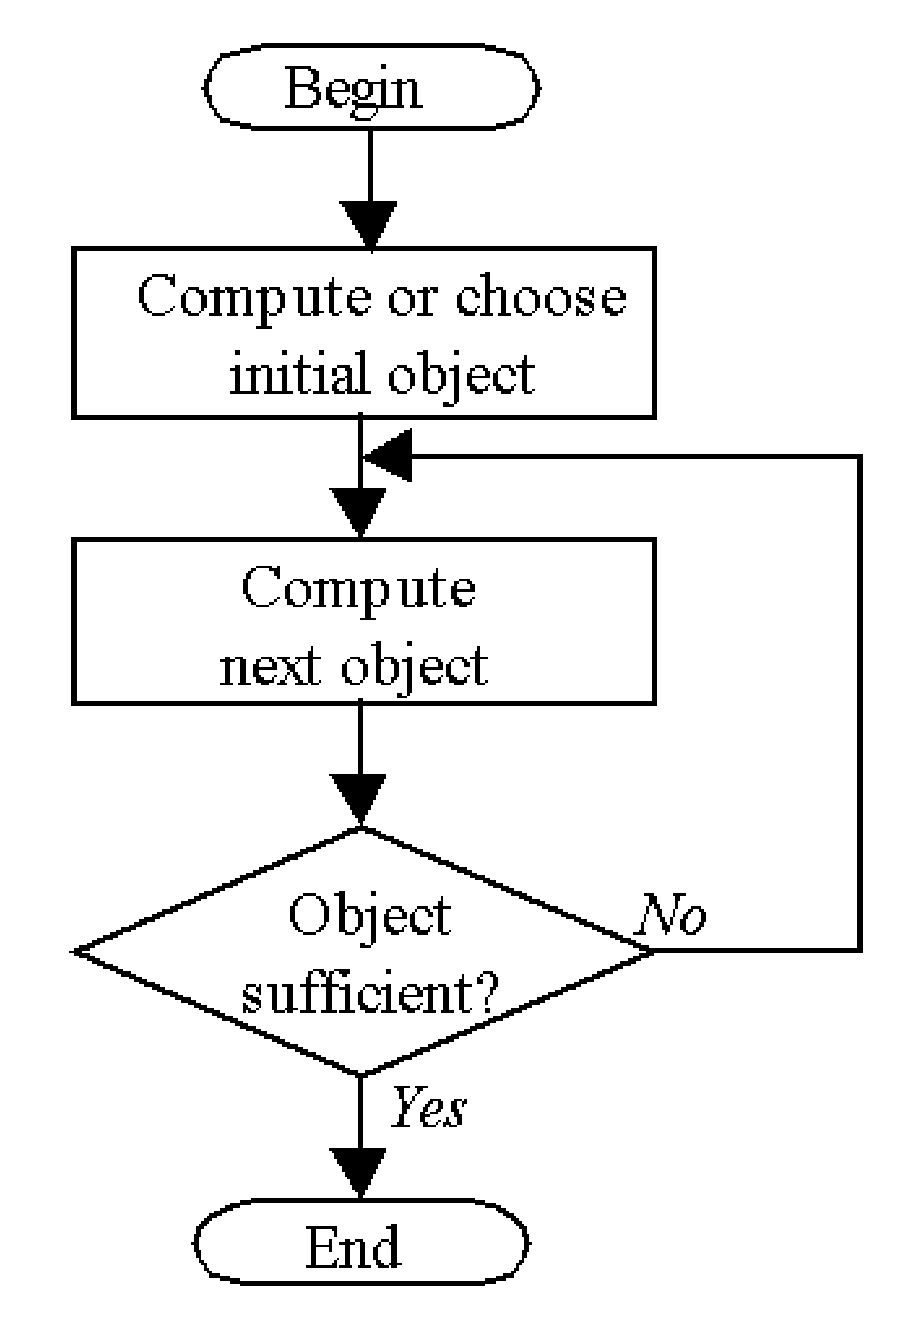
\includegraphics[width=5cm]{Figures/IterationCoarseFlow}
\caption{Successive approximation algorithm}\label{fig:itercoarse}
\end{figure}

The set-up phase allows determining constant parameters used by
the subsequent computations. Often a first estimation of the
solution is defined at this time. In any case an object
representing the approximate solution is constructed. Depending on
the complexity of the problem a class will explicitly represent
the solution object. Otherwise the solution shall be described by
a few instance variables of simple types (numbers and arrays).

After the set-up phase the iterative process proper is started. A
transformation is applied to the solution object to obtain a new
object. This process is repeated unless the solution object
resulting from the last transformation can be considered close
enough to the sought solution.

During the clean-up phase resources used by the iterative process
must be release. In some cases additional results may be derived
before leaving the algorithm.

\noindent Let us now explicit each of the three stages of the
algorithm.

The step computing or choosing an initial object is strongly
dependent on the nature of the problem to be solved. In some
methods, a good estimate of the solution can be computed from the
data. In others using randomly generated objects yields good
results. Finally, one can also ask the application's user for
directions. In many cases this step is also used to initialize
parameters needed by the algorithm.

The step computing the next object contains the essence of the
algorithm. In general a new object is generated based on the
history of the algorithm.

The step deciding whether or not an object is sufficiently close
to the sought solution is more general. If the algorithm is
capable of estimating the precision of the solution --- that is,
how close the current object is located from the exact solution
--- one can decide to stop the algorithm by comparing the
precision to a desired value. This is not always the case,
however. Some algorithms, genetic algorithms for example, do not
have a criterion for stopping.

Whether or not a well-defined stopping criterion exists, the
algorithm must be prevented from taking an arbitrary large amount
of time. Thus, the object implementing an iterative process ought
to keep track of the number of iterations and interrupt the
algorithm if the number of iterations becomes larger than a given
number.

\rubrique{Design}
%\marginpar{Figure \ref{cl:iteration} with the box {\bf IterativeProcess} grayed.}
Now we can add some details to the
algorithm. The new details are shown in figure \ref{fig:iterfine}.
\begin{figure}
\centering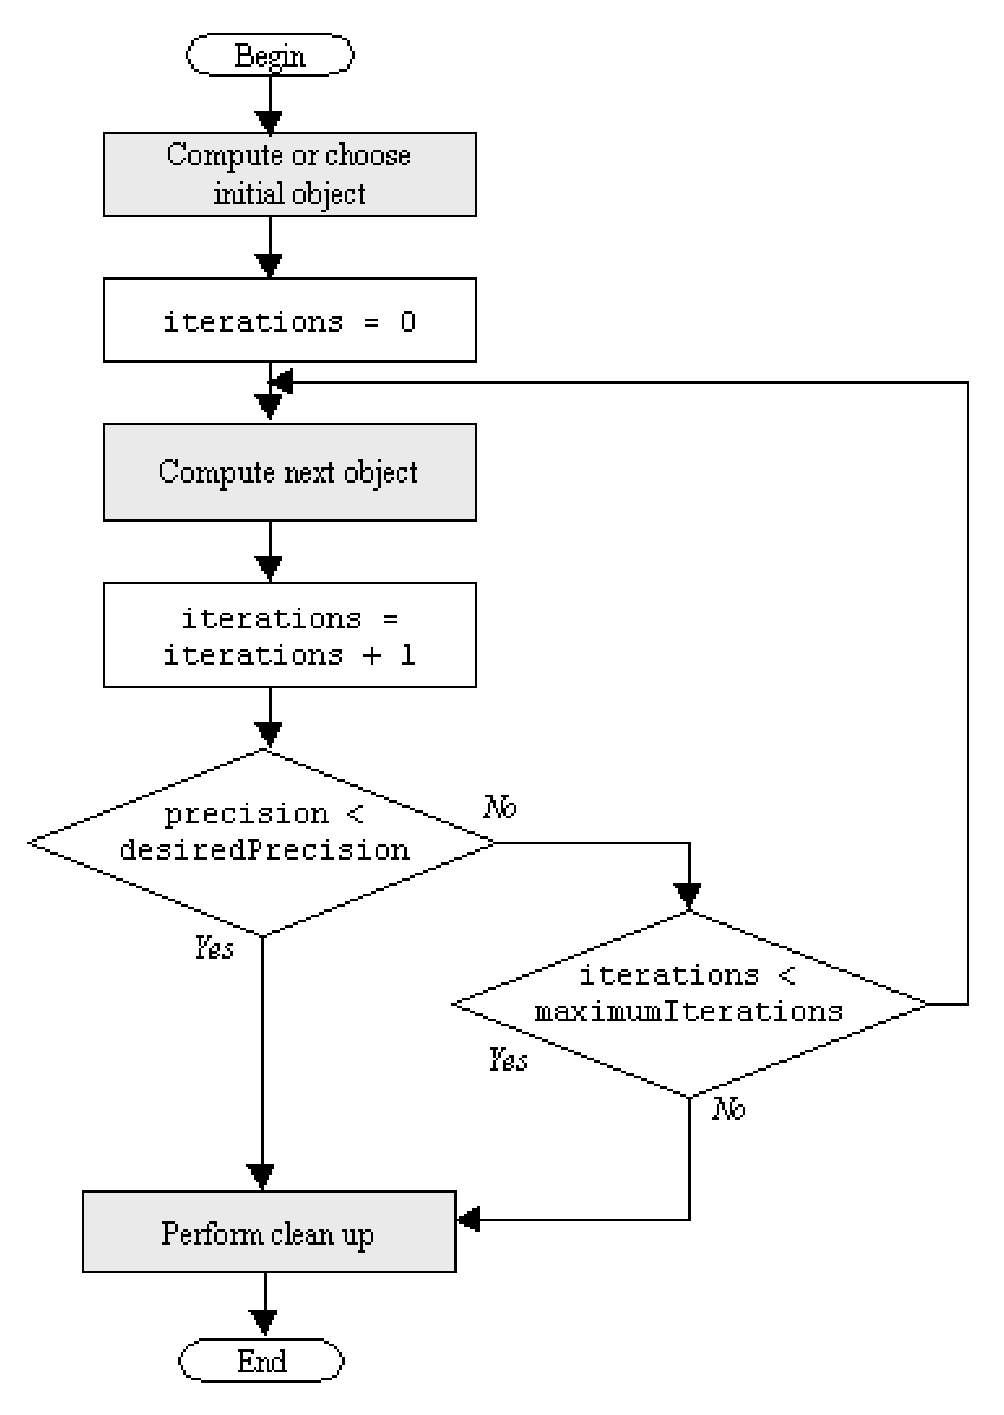
\includegraphics[width=4in]{Figures/IterationFineFlow}
\caption{Detailed algorithm for successive
approximations}\label{fig:iterfine}
\end{figure}
This schema allows us to determine the structure of a general
object implementing the iterative process. It will be implemented
as an abstract class. An abstract class is a class with does not
have object instances. A object implementing a specific algorithm
is an instance of a particular subclass of the abstract class.

The gray boxes in figure \ref{fig:iterfine} represent the methods,
which must be implemented explicitly by the subclass. The abstract
class calls them. However, the exact implementation of these
methods is not defined at this stage.
Such methods are called {\textsl hook} methods.

Using this architecture the abstract class is able to implement
the iterative process without any deep knowledge of the algorithm.
Algorithm specific methods are implemented by the subclass of the
abstract class.

Let us call \code{IterativeProcess} the class of the abstract
object. The class \code{IterativeProcess} needs the following
instance variables:
\begin{itemize}
\item \code{iterations}keeps track of the number of iterations, that is the number of successive
approximations,
\item \code{maximumIterations} maximum number of allowed iterations,
\item \code{desiredPrecision} the precision to attain, that is, how close to the solution should the solution object be when the algorithm is
terminated,
\item \code{precision} the precision achieved by the process. Its value is updated after each iteration and it is used to decide when to stop.
\end{itemize}
\begin{figure}
\centering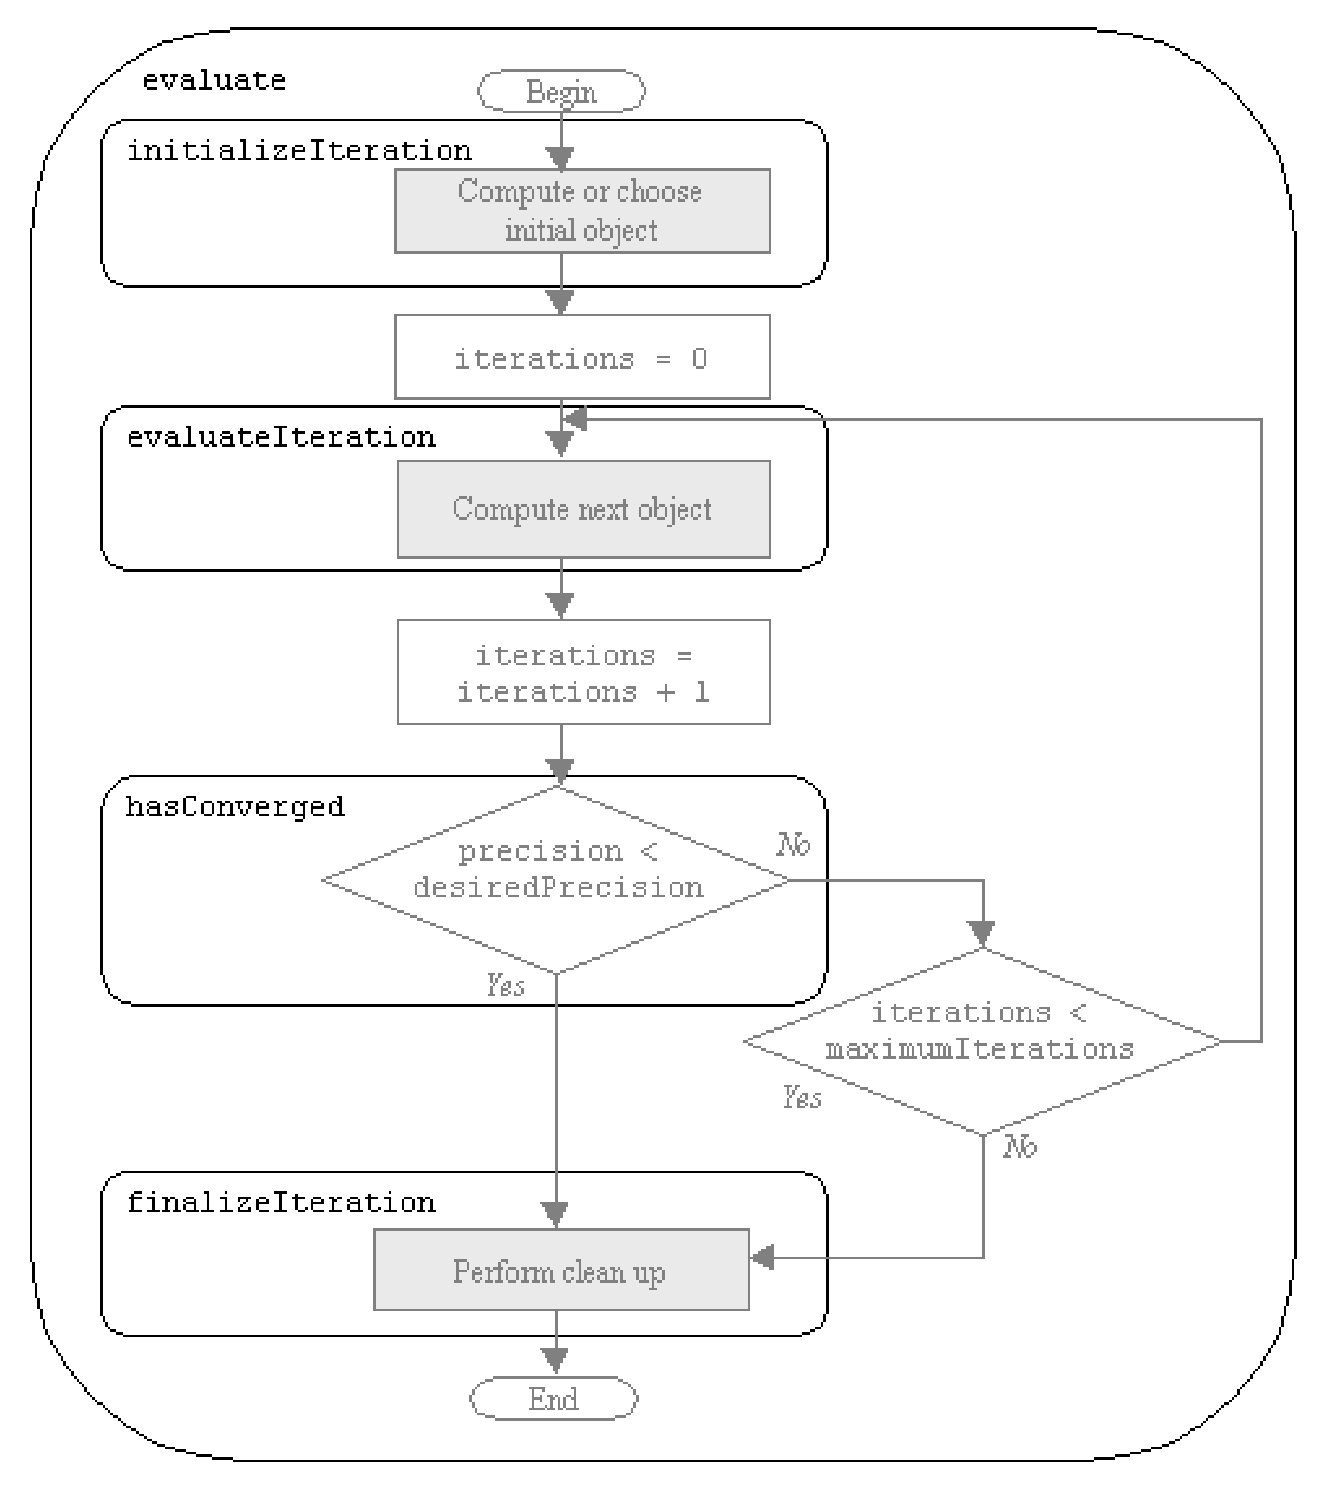
\includegraphics[width=4in]{Figures/IterationMethods}
\caption{Methods for successive
approximations}\label{fig:itermeth}
\end{figure}
The methods of the class \code{IterativeProcess} are shown in
figure \ref{fig:itermeth} in correspondence with the general
execution flow shown in figure \ref{fig:iterfine}. The two methods
\code{initializeIterations} and \code{finalizeIterations} should be
implemented by the subclass but the abstract class provides a
default behavior: doing nothing. The method \code{evaluateIteration} must be implemented by each subclass.

Since the precision of the last iteration is kept in an instance
variable, the method \code{hasConverged} can be called at any time
after evaluation, thus providing a way for client classes to check
whether the evaluation has converged or not.

\subsection{Iterative process --- Smalltalk implementation}
\label{sec:siteration}
Even though we are dealing for the moment
with an abstract class we are able to present a scenario of use
illustrating the public interface to the class. Here is how a
basic utilization of an iterative process object would look like.
\begin{displaycode}{Smalltalk}
| iterativeProcess result |
iterativeProcess := <a subclass of DhbIterativeProcess> new.
result := iterativeProcess evaluate.
iterativeProcess hasConverged
   ifFalse:[ <special case processing> ].
\end{displaycode}

The first statement creates an object to handle the iterative
process. The second one performs the process and retrieves the
result, whatever it is. The final statement checks for
convergence.

To give the user a possibility to have more control, one can
extend the public interface of the object to allow defining the
parameters of the iterative process: the desired precision and the
maximum number of iterations. In addition, the user may want to
know the precision of the attained result and the number of
iterations needed to obtain the result. The following code sample
shows an example of use for all public methods defined for an
iterative process. The precision of the attained result and the
number of iterations are printed on the transcript window.

\begin{displaycode}{Smalltalk}
| iterativeProcess result precision |
iterativeProcess := <a subclass of DhbIterativeProcess> new.
iterativeProcess desiredPrecision: 1.0e-6; maximumIterations: 25.
result := iterativeProcess evaluate.
iterativeProcess hasConverged
   ifTrue: [ Transcript nextPutAll: 'Result obtained after '.
             iterativeProcess iteration printOn: Transcript.
             Transcript nextPutAll: 'iterations. Attained precision is'.
             iterativeProcess precision printOn: Transcript.
             ]
    ifFalse:[ Transcript nextPutAll: 'Process did not converge'.].
Transcript cr.
\end{displaycode}

Listing \ref{lst:iteration} shows the Smalltalk implementation of the iterative process.

In the Smalltalk implementation, the class \code{IterativeProcess}
has one instance variable in addition to the ones described in the
preceding section. This variable, called \code{result}, is used to
keep the solution object of the process. The method \code{result}
allows direct access to it. Thus, all subclasses can use this
instance variable as a placeholder to store any type of result. As
a convenience the method \code{evaluate} also returns the instance
variable \code{result}.

Default values for the desired precision and the maximum number of
iterations are kept in class methods for easy editing. The method
initialize loads these default values for each newly created
instance. The default precision is set to the machine precision
discussed in section \ref{sec-rounding}.

The methods used to modify the desired precision (\code{desiredPrecision:}) and the maximum number of iterations (\code{maximumIterations:}) check the value to prevent illegal
definitions, which could prevent the algorithm from terminating.

Since there is no explicit declaration of abstract class and abstract methods in Smalltalk\footnote{An abstract class is a class containing at least an abstract method; an abstract method contains the single conventional statement: \code{self subclassResponsibility}} the three methods \code{initializeIterations}, \code{evaluateIteration} and \code{finalizeIterations}, are implemented with a reasonable default behavior.
The methods \code{initializeIterations} and \code{finalizeIterations} do nothing. The method \code{evaluateIteration} calls the method \code{subclassResponsibility}, which raises an
exception when called.
Using this technique is the Smalltalk way of creating an abstract method.
\begin{listing}[label=lst:iteration]{Smalltalk}
{Smalltalk implementation of an iterative process}
Object subclass: #PMIterativeProcess
   instanceVariableNames: 'precision desiredPrecision maximumIterations result iterations'
   classVariableNames: ''
   package: 'Math-Core-Process'
\end{listing}

\begin{displaycode}{Smalltalk}
PMIterativeProcess class >> defaultMaximumIterations
    ^50
\end{displaycode}

\begin{displaycode}{Smalltalk}
PMIterativeProcess class >> defaultPrecision
    ^PMFloatingPointMachine new defaultNumericalPrecision
\end{displaycode}

\begin{displaycode}{Smalltalk}
PMIterativeProcess >> desiredPrecision: aNumber
    aNumber > 0
        ifFalse: [ ^self error: 'Illegal precision: ', aNumber 
                                                         printString].
    desiredPrecision := aNumber.
\end{displaycode}

\begin{displaycode}{Smalltalk}
PMIterativeProcess >> evaluate
    iterations := 0.
    self initializeIterations.
    [iterations := iterations + 1.
    precision := self evaluateIteration.
    self hasConverged or: [iterations >= maximumIterations]] 
            whileFalse: [].
    self finalizeIterations.
    ^self result
\end{displaycode}

\begin{displaycode}{Smalltalk}
PMIterativeProcess >> evaluateIteration
    ^self subclassResponsibility
\end{displaycode}

\begin{displaycode}{Smalltalk}
PMIterativeProcess >> finalizeIterations
   "Perform cleanup operation if needed (must be implemented by subclass)."
\end{displaycode}

\begin{displaycode}{Smalltalk}
PMIterativeProcess >> hasConverged
    ^precision <= desiredPrecision
\end{displaycode}

\begin{displaycode}{Smalltalk}
PMIterativeProcess >> initialize
    desiredPrecision := self class defaultPrecision.
    maximumIterations := self class defaultMaximumIterations.
    ^self
\end{displaycode}

\begin{displaycode}{Smalltalk}
PMIterativeProcess >> initializeIterations
   "Initialize the iterations (must be implemented by subclass when needed)."
\end{displaycode}

\begin{displaycode}{Smalltalk}
PMIterativeProcess >> iterations
    ^iterations
\end{displaycode}

\begin{displaycode}{Smalltalk}
PMIterativeProcess >> maximumIterations: anInteger
    ( anInteger isInteger and: [ anInteger > 1])
        ifFalse: [ ^self error: 'Invalid maximum number of iteration: 
                                            ', anInteger printString].
    maximumIterations := anInteger
\end{displaycode}

\begin{displaycode}{Smalltalk}
PMIterativeProcess >> precision
    ^precision
\end{displaycode}

\begin{displaycode}{Smalltalk}
PMIterativeProcess >> precisionOf: aNumber1 relativeTo: aNumber2
    ^aNumber2 > PMFloatingPointMachine new defaultNumericalPrecision
        ifTrue: [ aNumber1 / aNumber2]
        ifFalse:[ aNumber1]
\end{displaycode}

\begin{displaycode}{Smalltalk}
PMIterativeProcess >> result
   ^result
\end{displaycode}

\begin{quote}
{\textbf Note:} The method \code{precisionOf:relativeTo:} implements
the computation of the relative precision. This is discussed in
section \ref{sec:siterrel}.
\end{quote}


\section{Evaluation with relative precision}
\label{sec:iterrel}
%\marginpar{Figure \ref{cl:iteration} with the box {\bf FunctionalIterator} grayed.}
So far we have made no
assumption about the nature of the solution searched by an
iterative process. In this section we want to discuss the case
when the solution is a numerical value.

As discussed in section \ref{sec-rounding} a floating-point number
is a representation with constant relative precision. It is thus
meaningless to use absolute precision to determine the convergence
of an algorithm. The precision of an algorithm resulting in a
numerical value ought to be determined relatively.

One way to do it is to have the method \code{evaluateIteration}
returning a relative precision instead of an absolute number.
Relative precision, however, can only be evaluated if the final
result is different from zero. If the result is zero, the only
possibility is to check for absolute precision. Of course, in
practice one does not check for equality with zero. The
computation of a relative precision is carried only if the
absolute value of the result is larger than the desired precision.

The reasoning behind the computation of the relative error is
quite general. Thus, a general-purpose class \code{FunctionalIterator} has been created to implement a method
computing the relative precision from an absolute precision and a
numerical result. In addition, since all subclasses of \code{FunctionalIterator} use a function a general method to handle the
definition of that function is also supplied.

\subsection{Relative precision --- Smalltalk  implementation}
\label{sec:siterrel} In this case the public interface is extended
with a creation method taking as argument the function on which
the process operates.
The code example of section \ref{sec:siteration} then becomes:
\begin{displaycode}{Smalltalk}
| iterativeProcess result |
iterativeProcess := <a subclass of PMFunctionalIterator>
                  function: ( PMPolynomial coefficients: #(1 2 3)).
result := iterativeProcess evaluate.
iterativeProcess hasConverged ifFalse:[ <special case processing>].
\end{displaycode}
In this example the function on which the process will operate is
the polynomial $3x^2+2x+1$ (\cf section \ref{sec:polynomial}).

Listing \ref{ls:iterrel} shows the implementation of the abstract
class \code{PMFunctionalIterator} in Smalltalk.

This class has one instance variable \code{functionBlock} to store
the function. A single class method allows creating a new instance
while defining the function.

As we have seen in section \ref{sec:stFunction}, a function can be
any object responding to the message value:. This allows supplying
any block of Smalltalk code as argument to the constructor method.
However, the user can also supply a class implementing the
computation of the function with a method with selector \code{value:}. For example, an instance of the class \code{PMPolynomial}
discussed in section \ref{sec:stPolynomial} can be used.

The instance method \code{setFunction:} is used to set the instance
variable \code{functionBlock}. In order to prevent a client class
from sending the wrong object, the method first checks whether the
supplied object responds to the message \code{value:}. This is one
way of ensuring that the arguments passed to a method conform to
the expected protocol. This way of doing is only shown as an
example, however. It is not recommend in practice. The
responsibility of supplying the correct arguments to a Smalltalk
method is usually the responsibility of the client class.

The method \code{initializeIterations} first checks whether a
function block has been defined. Then it calls the method \code{computeInitialValues}. This method is a hook method, which a
subclass must implement to compute the value of the result at the
beginning of the iterative process.

The computation of relative precision is implemented at two
levels. One general method, \code{precisionOf:relativeTo:},
implemented by the superclass allows the computation of the
relative precision relative to any value. Any iterative process
can use this method. The method \code{relativePrecision} implements
the computation of the precision relative to the current result.

\begin{listing}[label=lst:iterrel]{Smalltalk}
{Smalltalk implementation of the class PMFunctionalIterator}
PMIterativeProcess subclass: #PMFunctionalIterator
   instanceVariableNames: 'functionBlock'
   classVariableNames: ''
   package: 'Math-DHB-Numerical-Math-FunctionIterator'
\end{listing}

\begin{displaycode}{Smalltalk}
PMFunctionalIterator class >> function: aBlock
    ^self new setFunction: aBlock; yourself
\end{displaycode}

\begin{displaycode}{Smalltalk}
PMFunctionalIterator >> initializeIterations
    functionBlock isNil ifTrue: [self error: 'No function supplied'].
    self computeInitialValues
\end{displaycode}

\begin{displaycode}{Smalltalk}
PMFunctionalIterator >> relativePrecision: aNumber
    ^self precisionOf: aNumber relativeTo: result abs
\end{displaycode}

\begin{displaycode}{Smalltalk}
PMFunctionalIterator >> setFunction: aBlock
    ( aBlock respondsTo: #value:)
        ifFalse:[ self error: 'Function block must implement the 
                                                      method value:'].
    functionBlock := aBlock
\end{displaycode}

\section{Examples}
As we have dealt with abstract classes, this chapter did not give
concrete examples of use. By consulting the rest of this book the
reader will find numerous examples of subclasses of the two
classes described in this chapter. Table \ref{tb:iteration} lists
the sections where each algorithm using the iterative process
framework is discussed.
\begin{table}[h]
  \centering
  \caption{Algorithms using iterative processes}\label{tb:iteration}
\vspace{1 ex}
\begin{tabular}{|l|l|c|} \hline
\textbf{Algorithm or class of algorithm}&\textbf{Superclass}&\textbf{
Chapter or section}
\\ \hline Zero finding&Function iterator&Chapter \ref{ch:zeroes}
\\ \hline Integration&Function iterator&Chapter
\ref{ch:integration}
\\ \hline Infinite series and continued fractions&Function
iterator&Chapter \ref{ch:series}  \\ \hline Matrix
eigenvalues&Iterative process&Section \ref{sec:eigen}
\\ \hline Non-linear least square fit&Iterative process&Section
\ref{sec:lsfnonlin}
\\ \hline Maximum likelihood fit&Iterative process&Section \ref{sec:mlfhist} \\
\hline Function minimization&Function iterator&Chapter
\ref{ch:minimization}  \\ \hline Cluster analysis&Iterative
process&Section \ref{sec:cluster} \\ \hline
\end{tabular}

\end{table}

%\ifx\wholebook\relax\else\end{document}\fi
